\documentclass[border=1cm]{standalone}

\usepackage{tikz}
\usetikzlibrary{backgrounds}

\usepackage{xcolor}



\begin{document}

 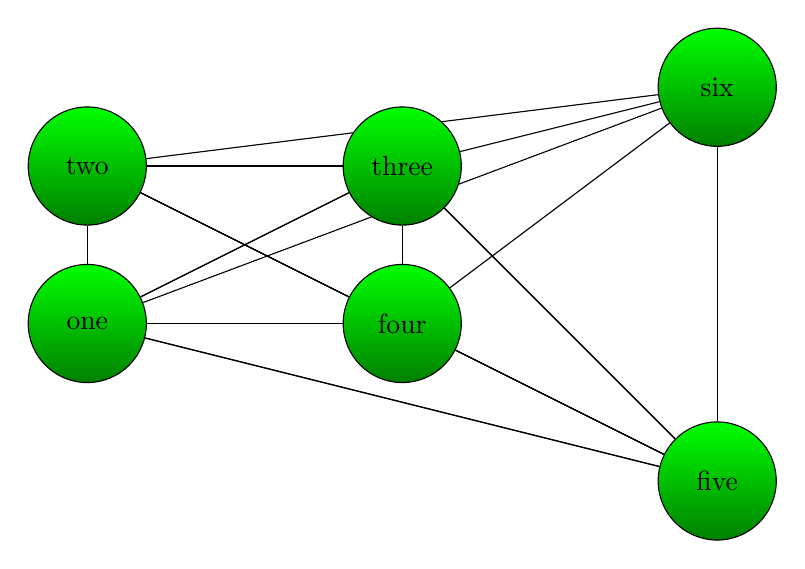
\begin{tikzpicture}[every node/.style={circle, fill=green,minimum width=15mm,draw,shading=axis,top color=green, bottom color=green!50!black}]

 \node (a) at (0,0){ one};
 \node (b) at (0,2) {two};
 \node (c) at (4,2) {three}; 
 \node (d) at (4,0) {four}; 
 \node (e) at (8,-2) {five}; 
 \node (f) at (8,3){six}; 


\begin{scope}[on background layer]
  \foreach \alpha in {a,b,c,d,e,f}%
  {%
  \foreach \alphb in {a,b,c,d,e}%
  {%
   \draw (\alpha) -- (\alphb);%
  }}
\end{scope}
 \end{tikzpicture}


\end{document}
